\documentclass{article}\raggedbottom

% if you need to pass options to natbib, use, e.g.:
% \PassOptionsToPackage{numbers, compress}{natbib}
% before loading nips_2016
%
% to avoid loading the natbib package, add option nonatbib:
% \usepackage[nonatbib]{nips_2016}

%\usepackage{nips_2016}

% to compile a camera-ready version, add the [final] option, e.g.:
% \usepackage[final]{nips_2016}

\usepackage[utf8]{inputenc} % allow utf-8 input
\usepackage[T1]{fontenc}    % use 8-bit T1 fonts
\usepackage[hidelinks]{hyperref}       % hyperlinks
\usepackage{url}            % simple URL typesetting
\usepackage{booktabs}       % professional-quality tables
\usepackage{amsfonts}       % blackboard math symbols
\usepackage{nicefrac}       % compact symbols for 1/2, etc.
\usepackage{microtype}      % microtypography
\usepackage{amsmath}
\usepackage{cleveref}
\usepackage{csvsimple}
\usepackage{graphicx}
\usepackage{color}
\usepackage{adjustbox}
\usepackage{float}

\title{Feature Selection in Finance, It is Delicious}
\usepackage[final]{nips_2016}

% The \author macro works with any number of authors. There are two
% commands used to separate the names and addresses of multiple
% authors: \And and \AND.
%
% Using \And between authors leaves it to LaTeX to determine where to
% break the lines. Using \AND forces a line break at that point. So,
% if LaTeX puts 3 of 4 authors names on the first line, and the last
% on the second line, try using \AND instead of \And before the third
% author name.

\author{
  Benjamin A. Schifman\\
  \textbf{Justin J. Siekmann}\\
  Department of Electrical and Computer Engineering\\
  University of Arizona\\
  Tucson, AZ 85719 \\
  \texttt{bschifman@email.arizona.edu} \\
  \texttt{jsiekmannemail.arizona.edu}
}

\begin{document}
 

\maketitle

\begin{abstract}
	\color{red}
  The abstract paragraph should be indented \nicefrac{1}{2}~inch
  (3~picas) on both the left- and right-hand margins. Use 10~point
  type, with a vertical spacing (leading) of 11~points.  The word
  \textbf{Abstract} must be centered, bold, and in point size 12. Two
  line spaces precede the abstract. The abstract must be limited to
  one paragraph.
\end{abstract}

\section{\color{red}Introduction}
There exist technical analysis indicators traditionally used by analysts to evaluate and predict market and equity performance. These indicators provide a unique perspective on the strength and direction of the underlying price action in market data. Feature selection is used to determine relevant indicators while identifying those that are irrelevant and redundant. Different implementations of algorithms based on these indicators could be used to predict performance of individual equities, sectors, or overall markets. They could also be used to classify and identify the correlation and interdependencies between equities, sectors, and markets. The goal of this paper is to implement various approaches to determine the efficacy of technical indicators as enablers to financial analysis. For analyzing features This project presented a couple challenges during implementation including developing an accurate testing method as well as handling and computing such large volumes of data.

Possibly reword and keep/move:\\
From this project we hope to deepen our understanding of the usage cases for applying specific machine learning algorithms as well as expanding upon our technical analysis of the stock market and which indicators play a role in successful market analysis.

\section{Related Work}
This is optional. If wanted, save til last.

\section{Methods/Approach}
The following subsections present details and explanations of the methods and functions implemented as part of this project.

\subsection{Data and Technical Analysis Indicators}
The Quandl platform was used to fetch 11 years of market data in total from Dec 31, 2006 to March 27, 2018 on various identified US tickers across different sectors. Tickers used in the project can be found in Table \ref{tab:tick} categorized by sector. As the process to fetch and preprocess the data is time consuming, pickle files were used to save data locally to be quickly reimported. TA-Lib: Technical Analysis Library was used to calculate features on the market data for each ticker. TA-Lib has the ability to calculate many technical analysis indicators in various categories. The features incorporated into this project, found with in \Cref{tab:inds}, are a selected subset of the indicators offered in TA-lib based upon the categories in TA-Lib, popularity online, and expert's favorites and essentials.

\begin{table}[h]
	\centering
	\csvautotabular{data/tickers.csv}
	\caption{Tickers}
	\label{tab:tick}
\end{table}

\begin{table}[h]
	\csvreader[respect all, autotabular, before reading=\begin{adjustbox}{max width=\columnwidth},after reading=\end{adjustbox}]{data/features_final.csv}{}{\csvlinetotablerow}
	\caption{Technical Analysis Indicators}
	\label{tab:inds}
\end{table}

\subsubsection{Indicator Categories}
  Overlap indicators generally can be overlayed onto the price charts. They most commonly include different styles of moving average calculations.
\\Momentum indicators convey how quickly the price of the ticker is moving. For example, the faster the price of a ticker increases the larger its momentum.
\\Volume indicators take into account the volume of the day's trading into account. 
\\Cycle indicators attempt to identify changes in the overall direction of the ticker's movement.
\\Price indicators combine the multiple prices in the data into one value.
\\Volatility indicators convey how sporadic the ticker's prices are.
\\Statistical indicators are based on statistical concepts and can be used in a number of different ways.
\\Math Transformation indicators apply common mathematical operations upon the tickers prices.
\\Pattern Recognition indicators look for patterns in the prices of a ticker traders have identified are indicative of future outcomes.

\subsection{Normalization}
As each technical analysis indicator produces values applicable based on how the indicator was calculated, normalization of the indicators makes correlations between them during feature selection more accurate and applicable. Each value is normalized using Equation \eqref{eq:norm}.

\begin{equation}\label{eq:norm}
	x_n = \frac{x - min}{max - min}
\end{equation}

\subsection{Feature Correlation}
Removing highly correlated features allows for the optimization of the classification algorithms by reducing the feature space. Features that are highly correlated most likely offer no additional data and they are an extra expense in computation time. The pairwise correlation of columns was computed, Figure~\ref{fig:corr_heatmap}.

\begin{figure}[h!]
	\centering
	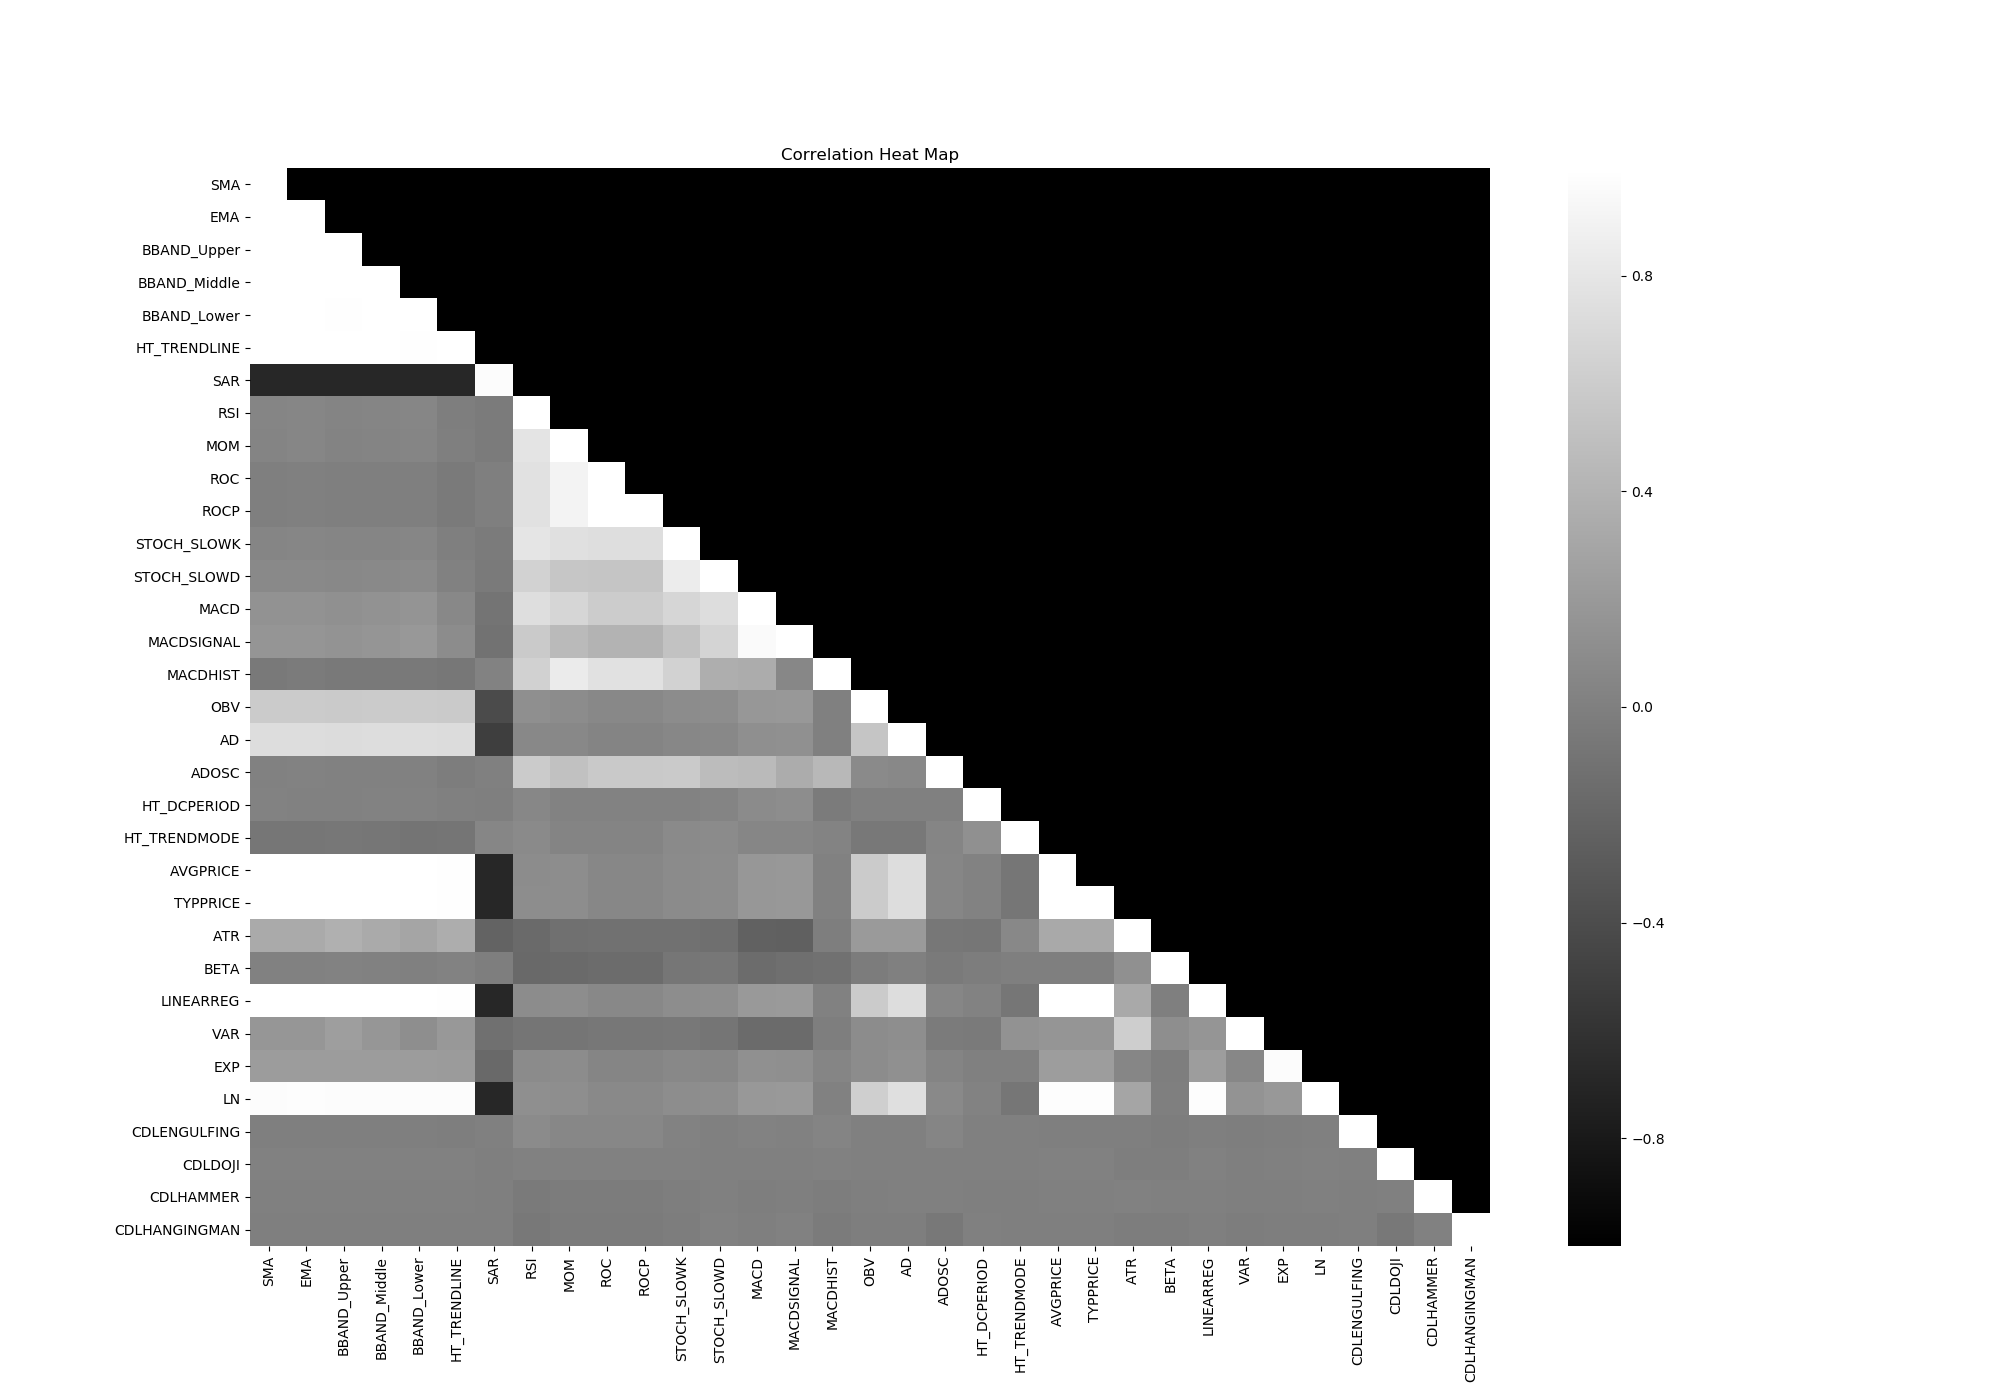
\includegraphics[width=\linewidth]{data/heatmapT1.png}
	\caption{Heat Map of Correlated Variables}
	\label{fig:corr_heatmap}
\end{figure}

\subsection{Maximal Information Coefficient (MIC)}\raggedbottom
The MIC is a measure of two-variable dependence designed specifically for rapid exploration of many-dimensional data sets \cite{reshef2011detecting}. A benefit to MIC correlations between two variables is that it can be described regardless of linear or non-linear relationships. The MIC yields a single vale $0 \leq MIC \leq 1$ with a value closer to $1$ representing that the variables are more closely correlated, and a value near $0$ indicates statistically independent variables that have neither linear nor nonlinear relationships. The $minepy$ library was used in python to rank the features according to their MIC with the target variable. The MIC was calculated for each feature in each ticker, yielding 33 MIC values for each ticker, and then a final set of MIC values were calculated by taking the ticker-wise mean over the MIC values.

\begin{figure}[H]
	\centering
	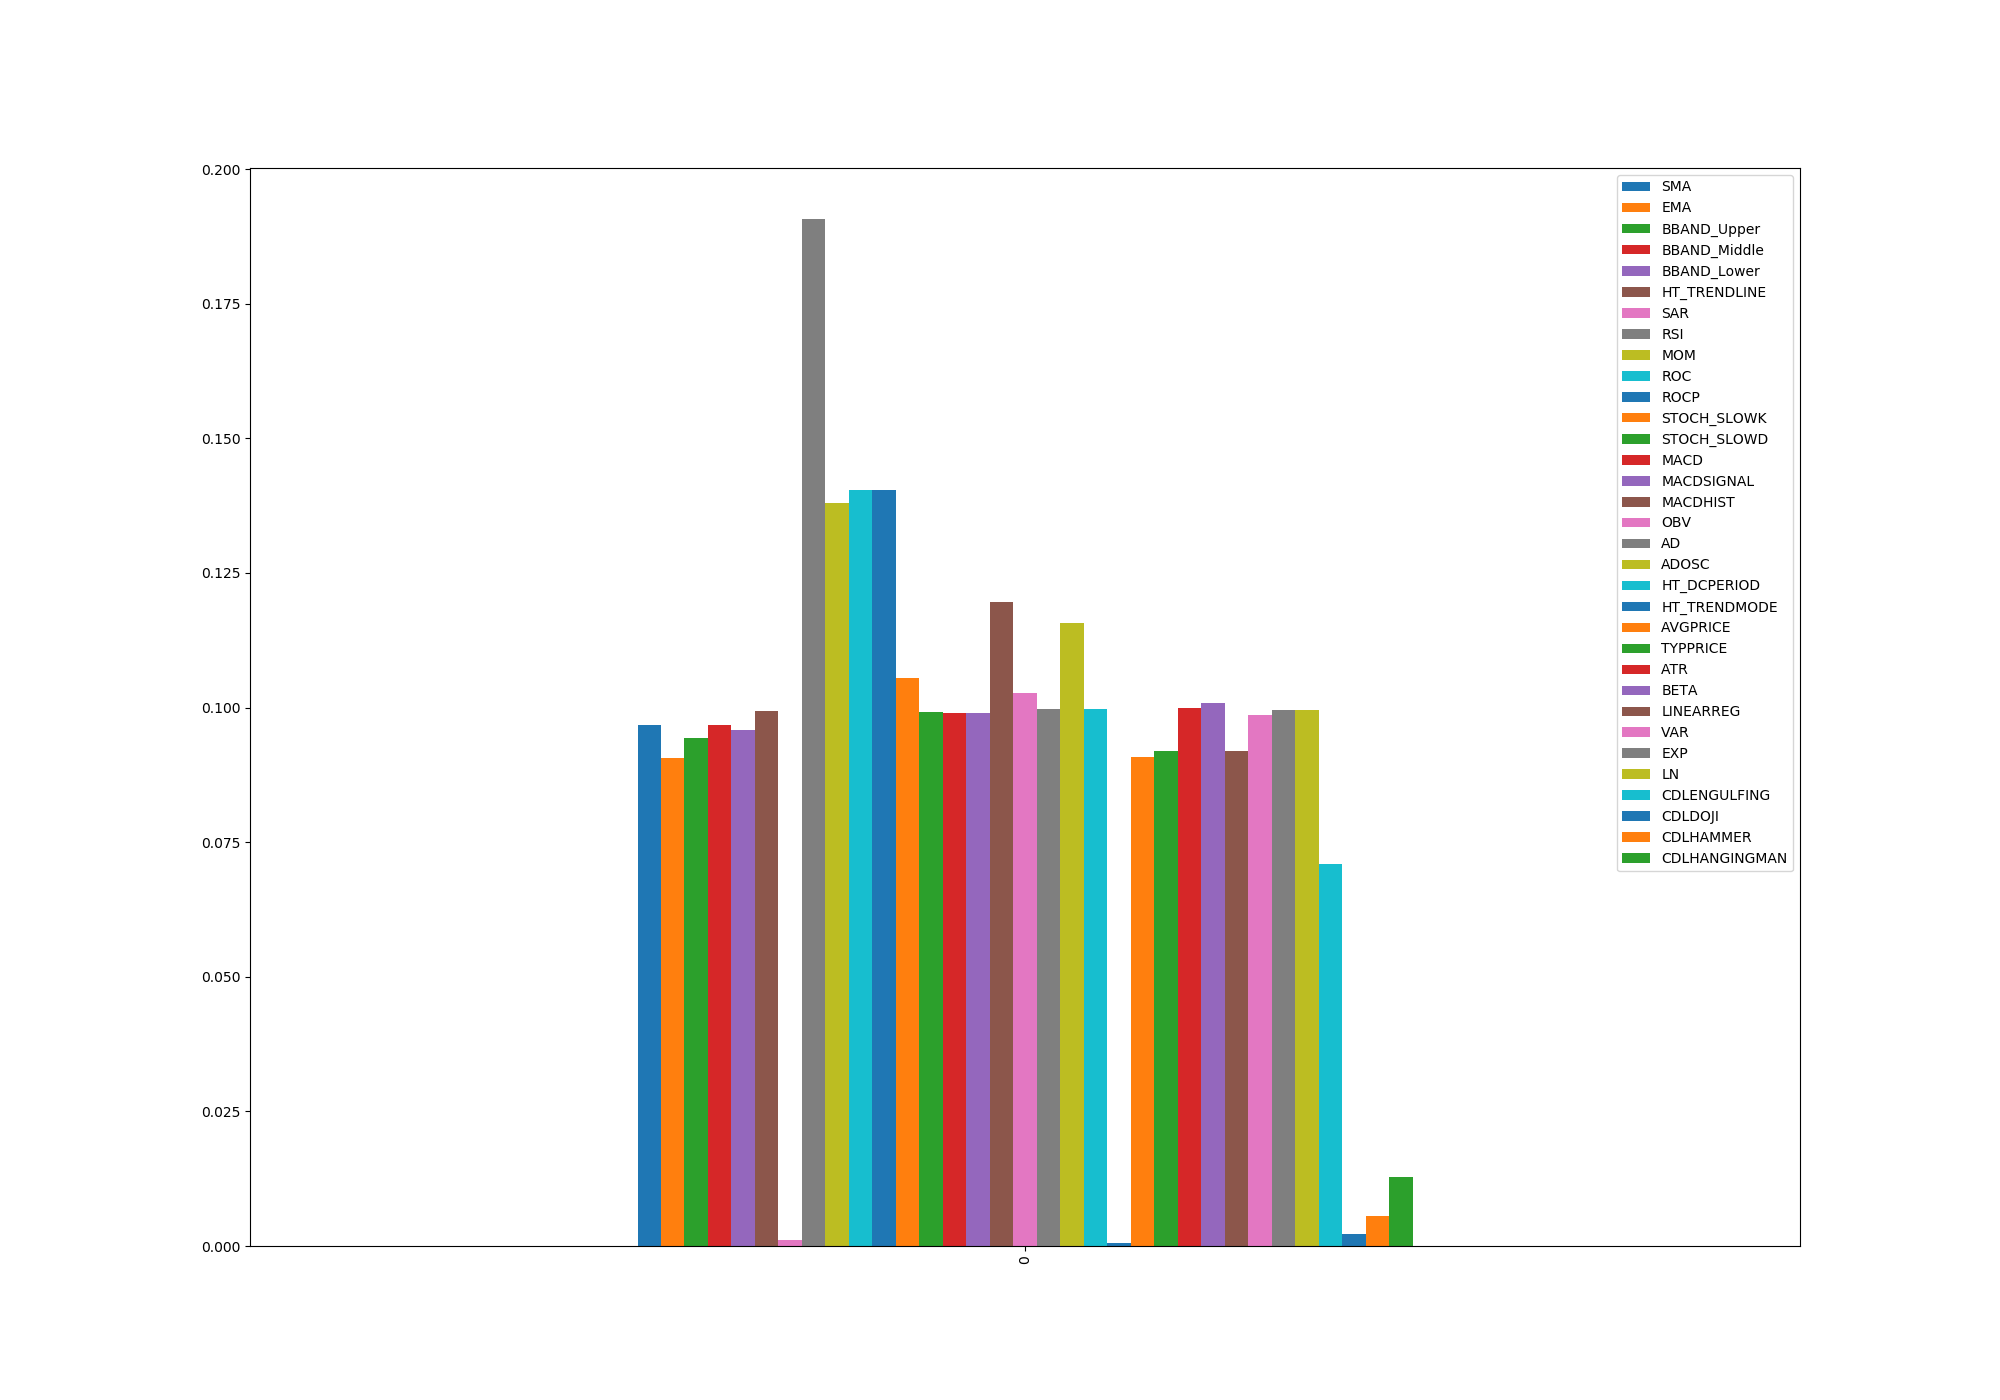
\includegraphics[width=\linewidth]{data/MICT1.png}
	\caption{Maximal Information Coefficient}
	\label{fig:MIC}
\end{figure}

\subsection{Recursive Feature Elimination (RFE)}
RFE is a method of recursively selecting smaller subsets of the larger feature set to then be used in an external classifier. The goal of RFE is to reduce the feature set into the smallest set of relevant and valuable features which yield the greatest accuracy. The time to run of the external classifier is reduced due to the fact that there are fewer features analyzed in the classification.
Given a base classifier, recursive feature elimination can be performed by re-training copies of the base classifier using a certain number of dropped features per iteration until the specified number of features to keep has been hit. RFE was implemented independently with two different base classifiers, SVM and Adaboosted Decision Trees.

\subsection{\color{red}Random Forest Classifier (RFC)}
The RFC is an ensemble algorithm implementing a combination of decision trees classifiers where the majority vote of all trees are used to classify the input feature vector \cite{pal2005random}. This RFC bagging method was used in order classify the input data, while also intrinsically implementing feature selection to return a vector of feature importances as depicted in Figure \ref{fig:RFC}. 

\begin{figure}[h!]
	\centering
	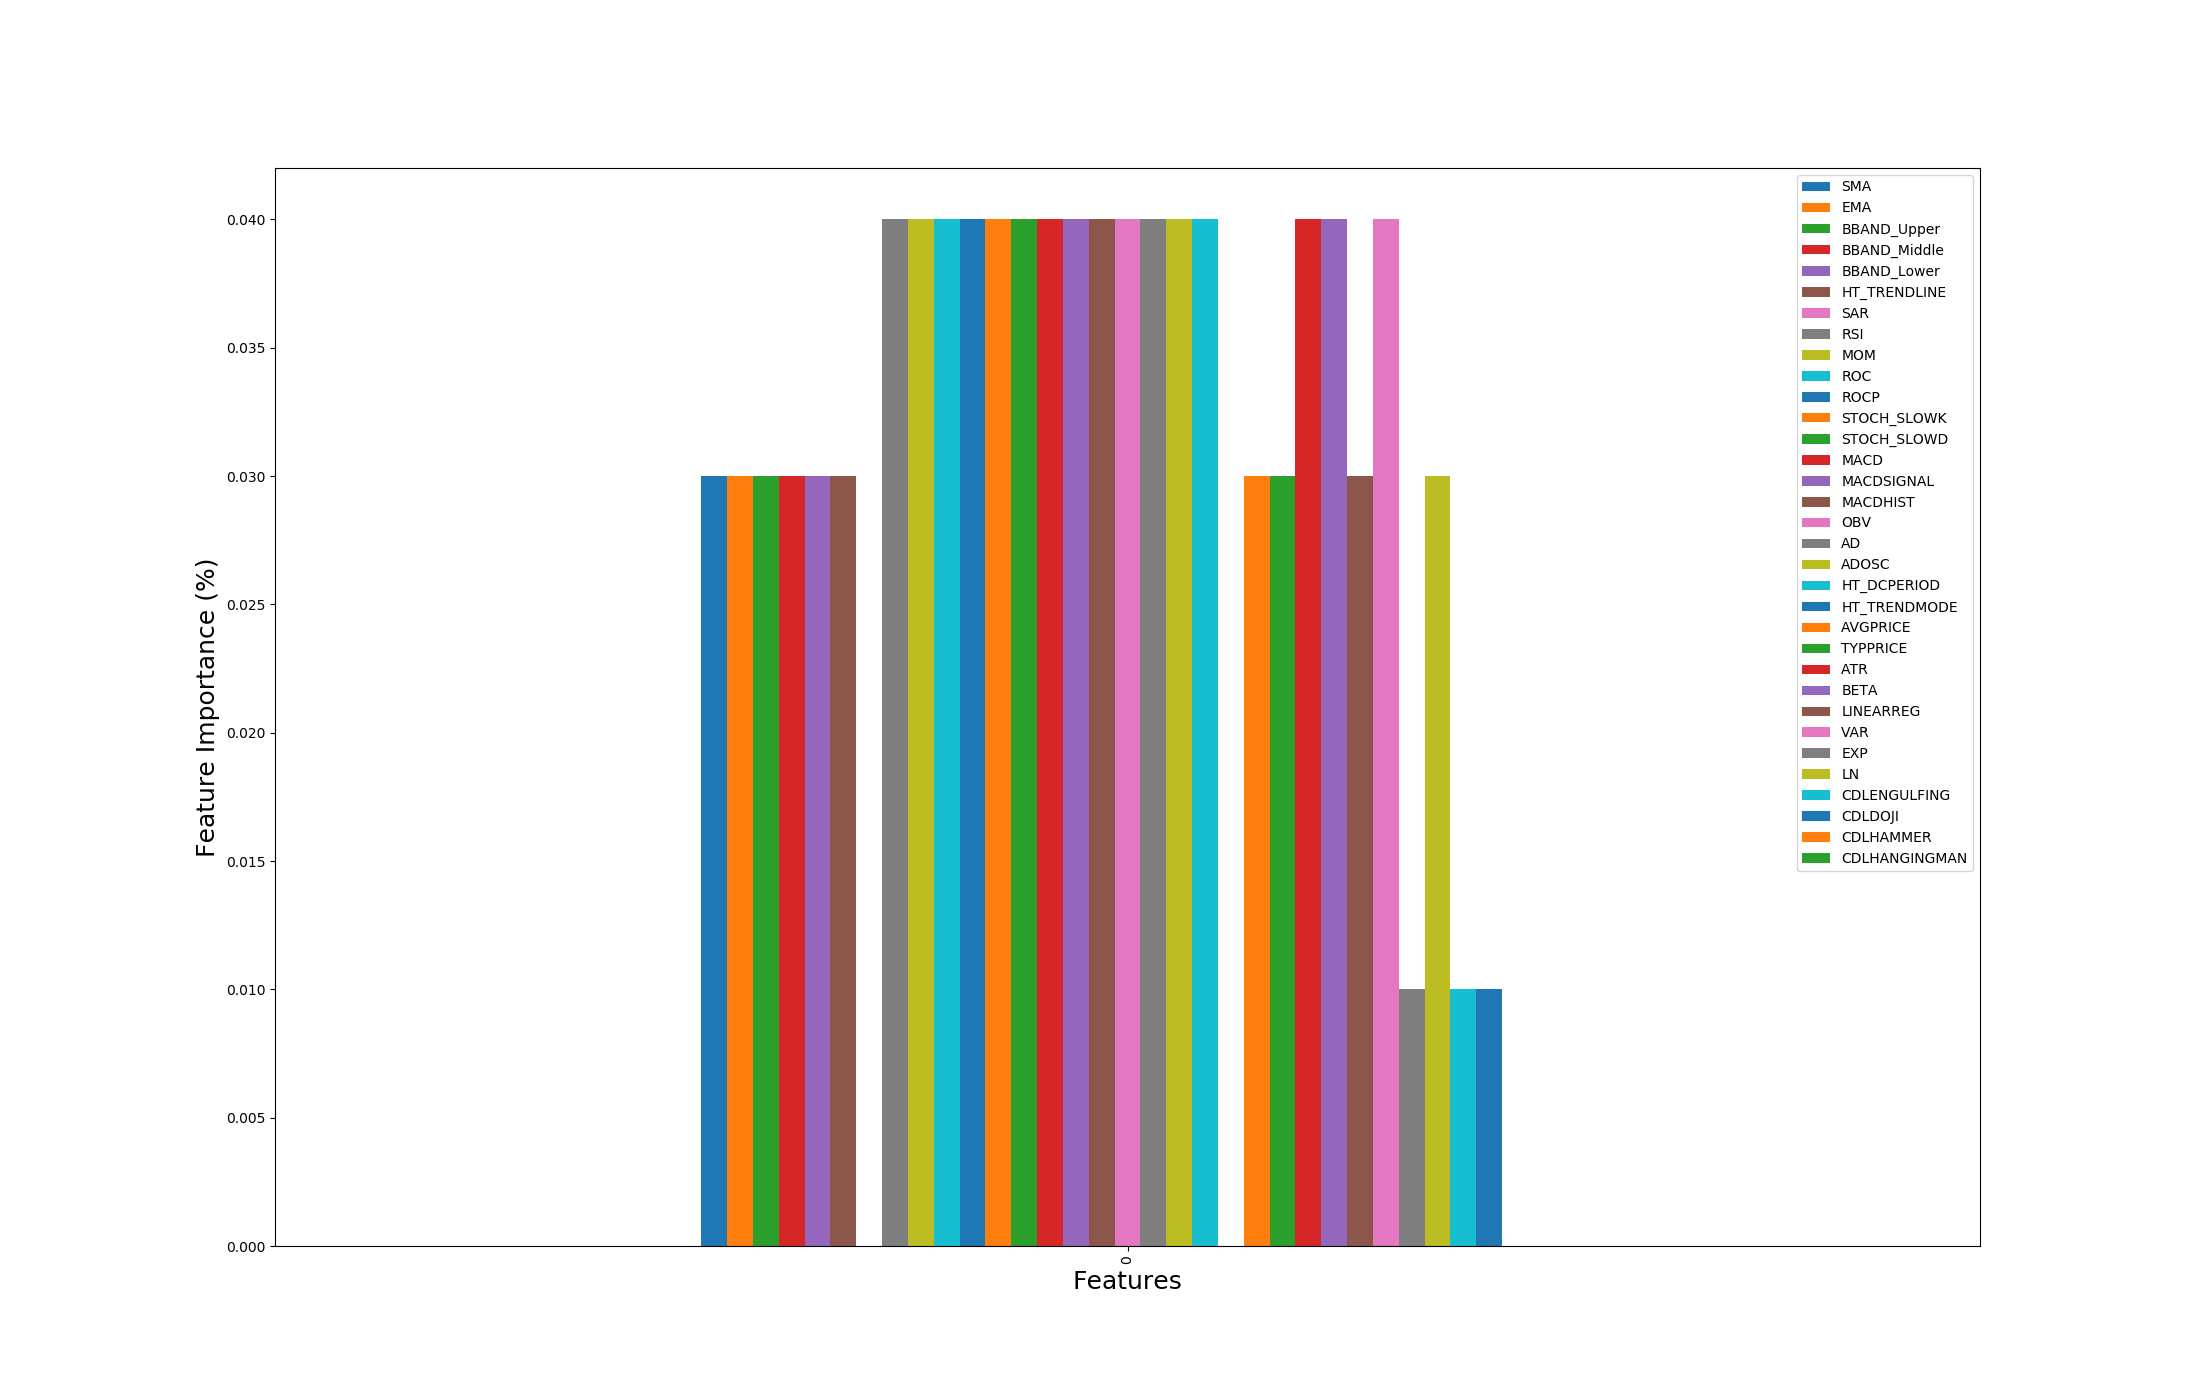
\includegraphics[width=\linewidth]{data/RFC_importancesT1.png}
	\caption{Random Forest Classifier}
	\label{fig:RFC}
\end{figure}

\subsection{Principal Component Analysis (PCA)}
PCA orthogonally transforms a set of features into a set of linearly uncorrelated principal components. PCA is a method for reducing the dimensionality of the feature set size while retaining principal component variance, and the features informational relevance. To analyze the performance of this method, PCA was implemented on the original 33 features and then the distilled principal components were used in the RFC classifier with 3 fold cross validation to determine the accuracy. The RFC classifier was used to analyze the validity of PCA because it intrinsically implements a form of feature selection as it weighs the features/principal components in terms of importance. The number of principal components the feature set was to be reduced to was iterated from 1 to 33 and then the accuracy of the RFC algorithm was calculated on each reduced feature set/principal component set. The following Figure \ref{fig:PCA} depicts the RFC accuracy and time taken with its corresponding reduced feature set of principal components.   

\begin{figure}[h!]
	\centering
	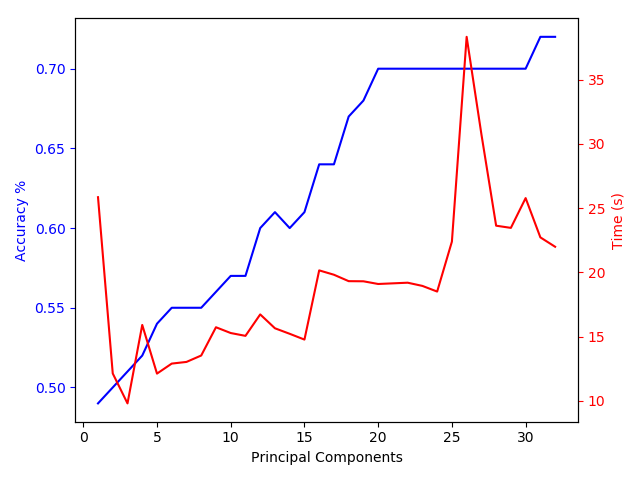
\includegraphics[width=\linewidth]{data/PCAT1.png}
	\caption{Principal Component Analysis}
	\label{fig:PCA}
\end{figure}

\section{Results}
Two testing sets were used to obtain results in this project. First the data was split into two sections. The first set consists of the majority of data (Dec 31, 2006 to Dec 31, 2016). This first set was randomly split using sklearn's train\_test\_split function to train and test each approach. Therefore the test set split from the first set is a collection of random days with the associated labels. The second set (Jan 1, 2017 to Mar 27, 2018) was only used in testing and tests performance day to day over a large chunk of time untouched by any training. As our random forest approach used cross fold validation test and retrain, this second data set was not used as a secondary test for our random forest or PCA approaches.
\subsection{Maximal Information Coefficient (MIC)}
\subsection{Recursive Feature Elimination (RFE)}


\begin{figure}[h!]
	\centering
	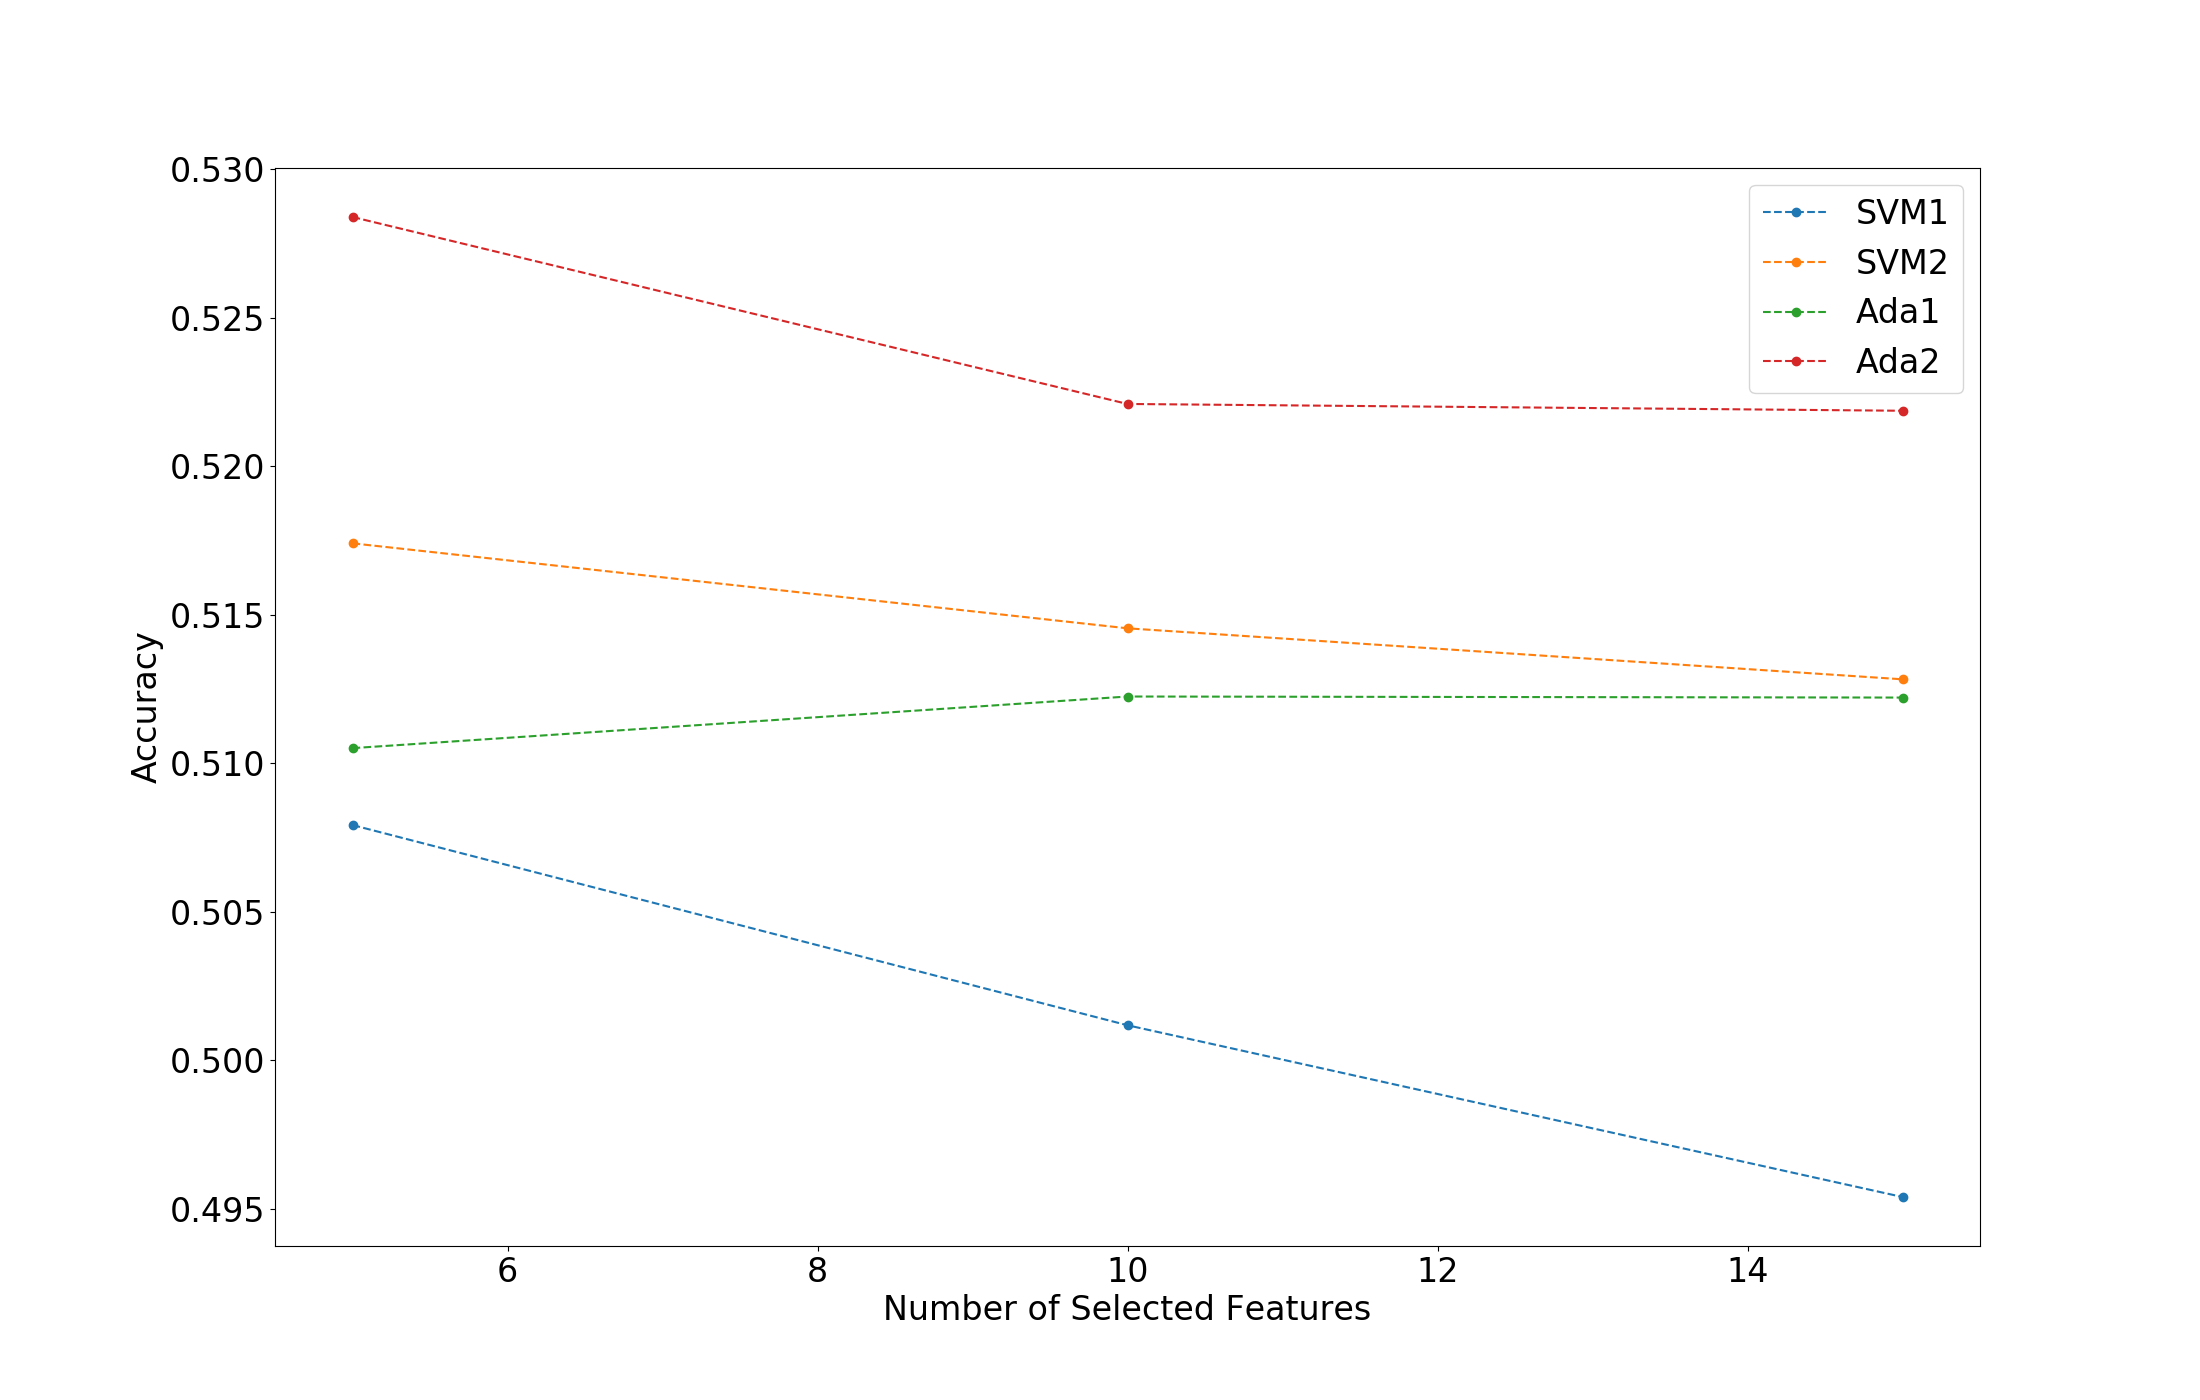
\includegraphics[width=\linewidth]{data/RFE.png}
	\caption{Recursive Feature Elimation Accuracies}
	\label{fig:RFE}
\end{figure}
\subsection{Random Forest Classifier (RFC)}
\subsection{Principal Component Analysis (PCA)}

\section{Conclusion}

%\section*{References}
\bibliography{bibfile} 
\bibliographystyle{unsrt}


\end{document}